\documentclass[12pt]{article}

\usepackage[left=.6in, right=.6in, top=0.75in, bottom=0.75in]{geometry}
\setlength\parindent{0pt}

\usepackage{graphicx, amsmath,anonchap,tabularx, multicol,array,graphbox}
\usepackage{cancel}
\usepackage{enumitem}
\setlist{noitemsep}
\setlist{nolistsep}
\usepackage{float}
\usepackage{multicol}

%\usepackage{draftwatermark}
%\SetWatermarkText{DRAFT}
%\SetWatermarkScale{5}
%\SetWatermarkColor[rgb]{0.8,0.8,0.8}
\newenvironment{boxe}
    {\begin{center}
    \begin{tabular}{|p{0.9\textwidth}|}
    \hline\\
    }
    { 
    \\\\\hline
    \end{tabular} 
    \end{center}
    }
    
\begin{document}

\begin{tabular*}{\textwidth}{@{\extracolsep{\fill}}l l}
\textbf{Name}\underline{\hspace{3in}}\\
\textbf{Math 160, Mean Value Theorem and Counter examples}  \\
\end{tabular*} \\

\vspace{.1in}
\small

\begin{enumerate}
    \item {\em Standard T2.} 
    
    Sketch a function that is continuous and differentiable on the interval $(-5,6)$ but is not defined at $x=-5$.

    \begin{center}
    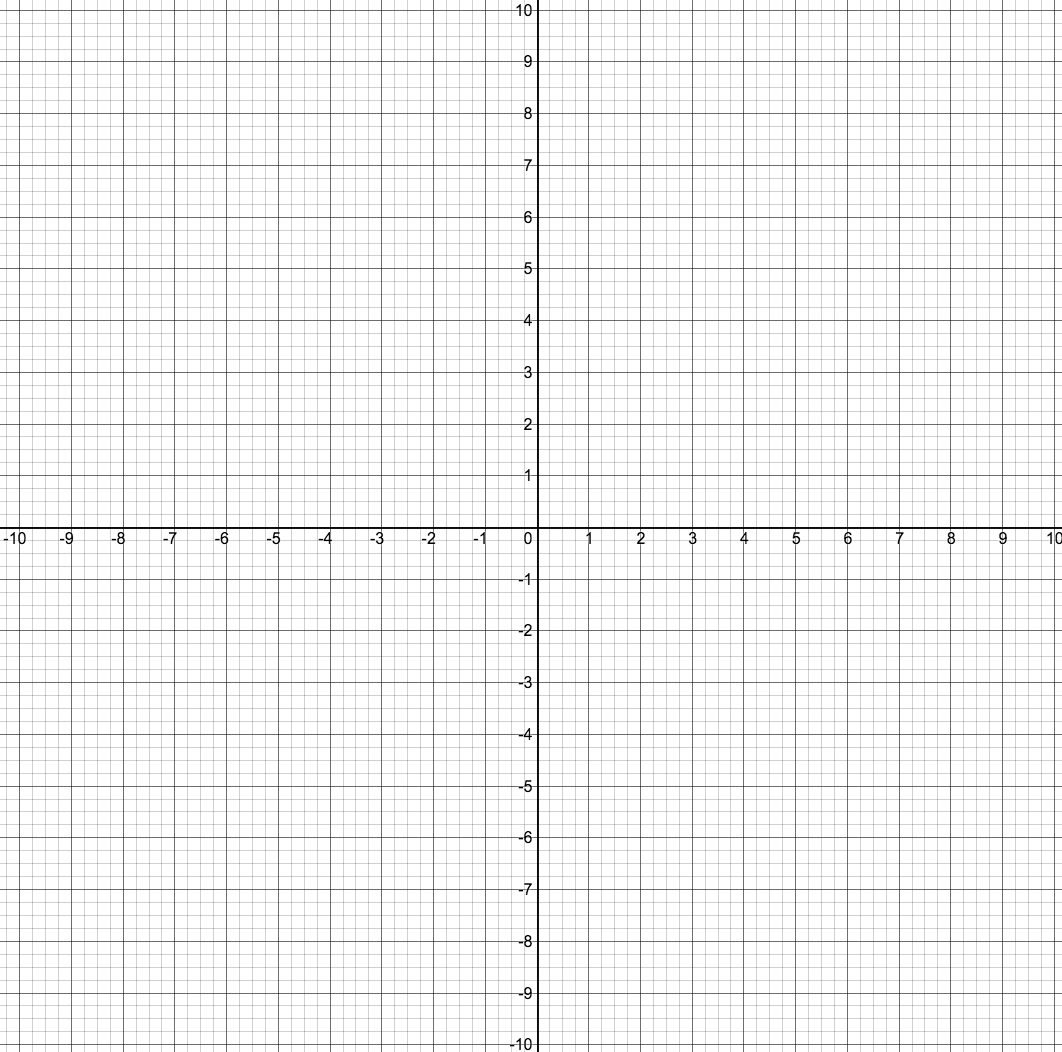
\includegraphics[width=0.5\textwidth, trim=120 0 0 0]{Axes2.png}
        
    \end{center}
    
    Now consider the statement: If a function $f$ is continuous and differentiable on $(a,b)$ then there exists a point $x=c$ on $(a,b)$ such that the slope of the tangent line at the point $x=c$ is equal to the slope of the secant line between $x=a$ and $x=b$.\\ 

    \begin{itemize}
        \item What is the difference between the Mean Value theorem and the statement above?\\\\\\
        \item Does your example satisfy the requirements for the above statement? Provide an interval and give a brief reasoning for each part.\\\\\\\\
        \item Does your example meet the conclusion of the statement above? If so what is the slope of the secant line and what is a $c$ value that works? If not explain what fails.\\\\\\\\
        \item Is your example a counterexample?
    \end{itemize}
    \newpage
    \item Create a counterexample for the following statement: Suppose $y=f(x)$ is continuous on $[a,b]$. Then there is at least one point $c$ in $(a,b)$ at which $\displaystyle{\frac{f(b)-f(a)}{b-a}=f'(c)}$.\\
    Make sure your answer includes all of the following: (i) A clearly defined function $f$ given graphically or with an equation. (ii) Specific values for $a$ and $b$. (iii) Show how the given function $f$, and the values $a$ and $b$ satisfy the hypothesis. (iv) Show how the conclusion is not satisfied.
    \vspace{4in}

    \begin{boxe}
        \textbf{The Mean Value Theorem:} Suppose $y=f(x)$ is continuous on $[a,b]$ and differentiable on $(a,b)$. Then there is at least one point $c$ in $(a,b)$ at which $\displaystyle{\frac{f(b)-f(a)}{b-a}=f'(c)}$
    \end{boxe}
    \item Let $v(x)=x^{x^x}-x^2$ which is continuous on $[0,\infty)$ and differentiable on $(0,\infty)$. Use the Mean Value Theorem to determine if there exists a point $x=c$ such that $v'(c)=0$ on the interval $(0,1)$

        
    
\end{enumerate}


\end{document}
